\documentclass[conference]{IEEEtran}
\IEEEoverridecommandlockouts
\usepackage{cite}
\usepackage{amsmath,amssymb,amsfonts}
\usepackage{algorithmic}
\usepackage{graphicx}
\usepackage{textcomp}
\usepackage{xcolor}
\usepackage{placeins}
\usepackage{float}
\usepackage[export]{adjustbox}
\usepackage{array}
\usepackage{stfloats}


\def\BibTeX{{\rm B\kern-.05em{\sc i\kern-.025em b}\kern-.08em
    T\kern-.1667em\lower.7ex\hbox{E}\kern-.125emX}}
\begin{document}

\title{PACT: Compliance Reporting in PPE Detection based on Pose-Anchored Body Region Assignment}

\makeatletter
\newcommand{\linebreakand}{%
  \end{@IEEEauthorhalign}
  \hfill\mbox{}\par
  \mbox{}\hfill\begin{@IEEEauthorhalign}
}
\makeatother

\author{
  \IEEEauthorblockN{1\textsuperscript{st} Given Name Surname}
  \IEEEauthorblockA{\textit{dept. name of organization (of Aff.)} \\
    \textit{name of organization (of Aff.)}\\
    City, Country \\
    email address}
  \and
  \IEEEauthorblockN{2\textsuperscript{nd} Given Name Surname}
  \IEEEauthorblockA{\textit{dept. name of organization (of Aff.)} \\
    \textit{name of organization (of Aff.)}\\
    City, Country \\
    email address}
  \and
  \IEEEauthorblockN{3\textsuperscript{rd} Given Name Surname}
  \IEEEauthorblockA{\textit{dept. name of organization (of Aff.)} \\
    \textit{name of organization (of Aff.)}\\
    City, Country \\
    email address}
  \linebreakand % <------------- \and with a line-break
  \IEEEauthorblockN{4\textsuperscript{th} Given Name Surname}
  \IEEEauthorblockA{\textit{dept. name of organization (of Aff.)} \\
    \textit{name of organization (of Aff.)}\\
    City, Country \\
    email address}
  \and
  \IEEEauthorblockN{5\textsuperscript{th} Given Name Surname}
  \IEEEauthorblockA{\textit{dept. name of organization (of Aff.)} \\
    \textit{name of organization (of Aff.)}\\
    City, Country \\
    email address}
}


\maketitle{}

\begin{abstract}
Automated systems that detect personal protective equipment (PPE) in images typically report only scene-level presence, failing to assign each item to a specific worker and preventing per-worker compliance checks required by safety regulations. This paper addresses this gap with Pose-Anchored Compliance Tracker (PACT), a three-stage pipeline. First, a YOLO26L detector locates PPE items and a YOLOv8x-pose model identifies workers and body keypoints. Second, a pose-anchored matching module attributes each detected PPE instance to the corresponding person. Third, a rule-based reporter computes fractional compliance scores and severity-tiered violation notices for each worker. We evaluate on three public datasets: construction-site CHV, medical PPE CPPE-5, and industrial SH17. PACT achieves mean average precision at IoU 0.50 (mAP\textsubscript{50}) of 0.923 on CHV and 0.652 on SH17, while per-person assignment accuracy reaches 0.938 on CHV and 0.892 on SH17. These results demonstrate that pose estimation enables reliable person-level PPE attribution and that assignment accuracy is a measurable target for compliance reporting.
\end{abstract}


\begin{IEEEkeywords}
PPE,
Compliance reporting,
Pose Estimation,
YOLOv8-pose,
YOLO26
\end{IEEEkeywords} 



\section{Introduction}
Occupational safety regulations including Occupational Safety and Health Administration (OSHA) 29 CFR 1926 \cite{OSHA_CFR1926}, ANSI/ISEA 107-2020 \cite{ANSI_ISEA107}, and ISO 45001 \cite{ISO45001} mandate the use of personal protective equipment (PPE) across construction, manufacturing, and healthcare environments. Non-compliance contributes to preventable workplace injuries, while manual inspection is neither scalable nor consistently reliable in large and dynamic work sites \cite{ref6}. Automated reporting through computer vision has therefore emerged as a practical alternative for continuous PPE verification.

Current approaches treat PPE compliance as an object detection problem, applying YOLO-based detectors to construction CHV \cite{ref5}, manufacturing SH17 \cite{ref2}, and medical CPPE-5 \cite{ref1} datasets. Detection-only systems produce PPE bounding boxes without associating each item to a specific worker, making per-person compliance evaluation impossible in multi-person scenes. Some works incorporate pose estimation to filter false positives \cite{ref8},\cite{ref12},\cite{ref13} but pose is used strictly as a preprocessing step. None of these works define PPE-to-person assignment as an explicit task or produce per-person compliance scores. Vukicevic et al.\ \cite{ref6} identify this as an open problem, noting that practical compliance systems require joint handling of human identification, pose estimation, and object recognition.

This work presents Pose-Anchored Compliance Tracker (PACT), a three-stage pipeline consisting of parallel YOLO26L \cite{sapkota_yolo26_2026} detection and YOLOv8x-pose estimation \cite{yaseen_what_2024}, followed by a pose-anchored PPE-to-person assignment module and a rule-based per-person compliance reporting mechanism. PACT formalizes PPE-to-person assignment as an explicit evaluation task by introducing a dedicated assignment accuracy metric for multi-person scenarios. A multi-stage evaluation protocol independently quantifies person detection, PPE detection, and assignment accuracy across 10,458 images.



\section{Related Work}


\subsection{PPE Detection and Pose-Assisted Compliance}

\begin{figure*}[!b]
    \centering
    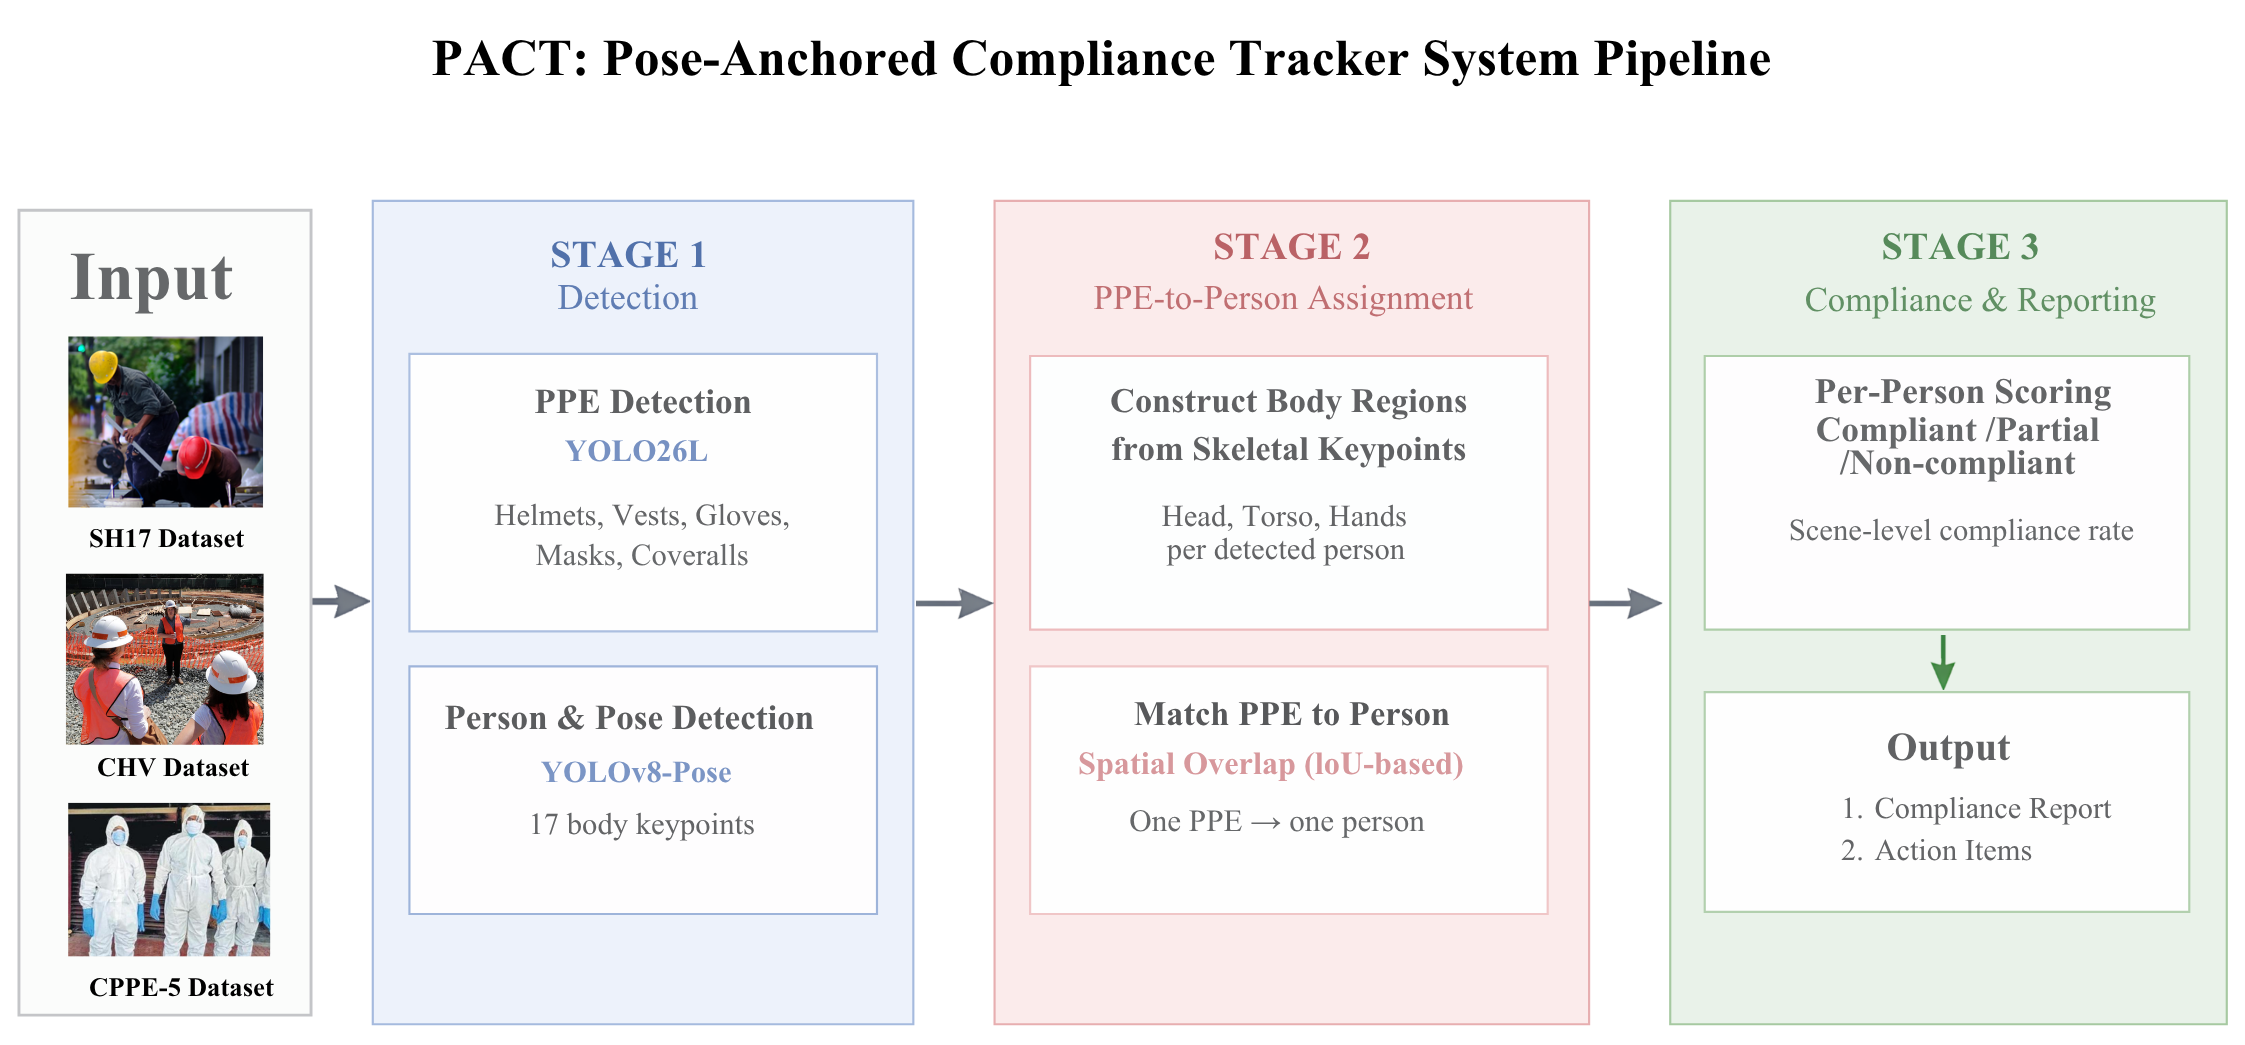
\includegraphics[width=\textwidth]{figures/pipeline.png}
    \caption{Overview of the PACT pipeline showing parallel PPE detection and pose estimation, followed by pose-anchored assignment and per-person compliance reporting.}
    \label{fig:pipeline}
\end{figure*}

\begin{table*}[!t]
\centering
\caption{Comparison of Representative PPE Compliance Methods (with Datasets)}
\label{tab:related_comparison}
\renewcommand{\arraystretch}{1.2}
\resizebox{\linewidth}{!}{%
\begin{tabular}{lllllccccc}
\hline
\textbf{Method} &
\textbf{Publication Year} &
\textbf{Detector} &
\textbf{Domain} &
\textbf{Dataset} &
\makebox[1.1cm]{\textbf{Pose Usage}} &
\textbf{Per-Person} &
\makebox[1.5cm]{\textbf{Compliance Type}} &
\makebox[1.2cm]{\textbf{Severity Report}} &
\textbf{Performance} \\
\hline
Wang et al.~\cite{ref5}
 & 2021 & YOLOv5 & Construction & GDUT‑Hardhat (custom) & None & No & -- & No & mAP 0.866 (YOLOv5x) \\
Gong et al.~\cite{ref13}
 & 2021 & YOLOv3 + ResNet50 & Offshore & Custom offshore platform & ROI & Yes & Binary & No & Helmet 94.8\% / Workwear 95.4\% \\
Gallo et al.~\cite{ref14}
 & 2022 & YOLOv4 & Industrial & PICTOR & None & No & -- & No & mAP 0.863 / 6.8 FPS \\
Vukicevic et al.~\cite{vukicevic2022compliance}
 & 2022 & YOLOv5 & Industrial & Custom head‑mounted images & ROI & Yes & Binary & No & Precision 0.920 / Recall 0.611 \\
Ahmed et al.~\cite{ref23}
 & 2023 & Faster R‑CNN & General & Mixed public + web‑scraped & None & Single & -- & No & mAP 0.960 \\
Kisaezehra et al.~\cite{ref9}
 & 2023 & YOLOv5 & Construction & Construction images (Roboflow) & None & No & -- & No & mAP 0.958 / 70.4 FPS \\
Monnikhof et al.~\cite{ref8}
 & 2023 & YOLOv7 + pose model & Custom & Custom pipeline recordings & Filter & No & -- & No & FP reduction 0.22 \\
Imam et al.~\cite{ref12}
 & 2024 & YOLOv8-pose + YOLOv8l & Mining & Self‑collected underground mine & Filter & Yes & Binary & No & Pose mAP 0.90 / PPE mAP 0.97 \\
Wen et al.~\cite{wen_automated_2024}
 & 2024 & YOLO + VQA & Construction & Custom construction VQA & None & No & Scene & No & Not reported \\
\hline
\multicolumn{10}{p{\linewidth}}{\scriptsize
\textbf{Pose Usage:} None = not used; ROI = keypoint-defined detection regions; Filter = false-positive suppression. \enspace
\textbf{Per-Person:} Single = evaluated on single-person images only. \enspace
\textbf{Compliance Type:} Binary = pass/fail per person, Scene = scene-level label, Fractional = continuous per-person score, -- = not reported. \enspace
\textbf{Severity Report:} Yes = severity-tiered corrective action report provided. \enspace
All mAP values are at IoU 0.50 unless stated otherwise.}
\end{tabular}}
\end{table*}

Single-stage YOLO detectors have become the dominant approach for PPE compliance due to their accuracy and low latency \cite{ref6}. Wang et al.\ introduced the CHV dataset and benchmarked eight YOLO variants, with YOLOv5x achieving 0.866 mAP \cite{ref5}; Kisaezehra et al.\ reported 0.958 mAP and 70.4~FPS on helmet detection using YOLOv5 variants \cite{ref9}. Gallo et al. demonstrated real-time edge deployment using lightweight CNNs \cite{ref14}. Two-stage detectors have also been explored: Ahmed et al.\ achieved 0.96 mAP with Faster R-CNN on eight PPE classes but were limited to single-person evaluation \cite{ref23}. Across these works, detection is treated as a class-presence problem: the system confirms whether a PPE category exists in the scene without attributing items to specific workers.

Recent works incorporate pose estimation to reduce false positives. Monnikhof et al.\ used YOLO-pose keypoints as anatomical constraints to filter implausible detections, reducing false positives by 0.22 \cite{ref8}. Imam et al.\ applied YOLOv8-pose to discard unlinked PPE detections in mining environments \cite{ref12}, and Gong et al.\ defined keypoint-based ROIs before PPE classification \cite{ref13}. Despite improved precision, pose is used solely as a post-detection filter in all cases; none formalize PPE-to-person assignment as an explicit task or evaluate per-person attribution in multi-worker scenes. Vukicevic et al.\ identify this as an open problem, noting that practical systems must jointly address detection, pose estimation, and assignment \cite{ref6}. This gap is the primary motivation for the proposed framework.

\begin{table*}[!b]
\centering
\caption{Qualitative Results of the Proposed PACT Framework}
\label{tab:qualitative_results}
\footnotesize
\setlength{\tabcolsep}{3pt}
\renewcommand{\arraystretch}{1.5}

\begin{tabular}{
p{0.08\textwidth}
>{\centering\arraybackslash}p{0.22\textwidth}
>{\centering\arraybackslash}p{0.22\textwidth}
>{\centering\arraybackslash}p{0.22\textwidth}
>{\centering\arraybackslash}p{0.22\textwidth}
}
\hline
\textbf{Dataset} & \textbf{Raw} & \textbf{Pose} & \textbf{Pose + PPE Detection} & \textbf{Report} \\
\hline

% Baris CHV
\rule{0pt}{10pt} % Memberi sedikit ruang di atas teks
\textbf{CHV} &
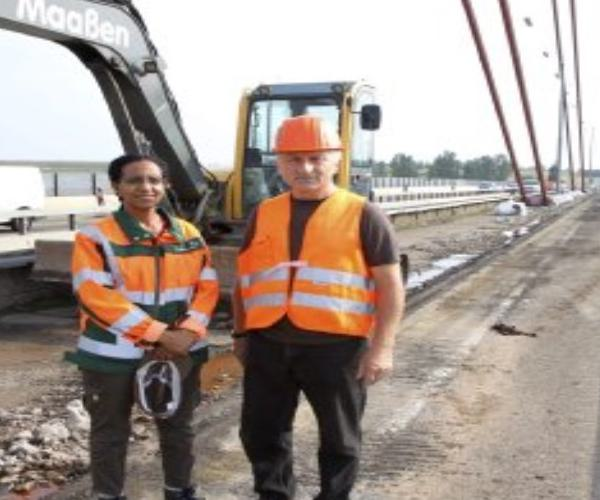
\includegraphics[width=\linewidth, valign=t]{figures/raw1_crop_600x500.jpg} &
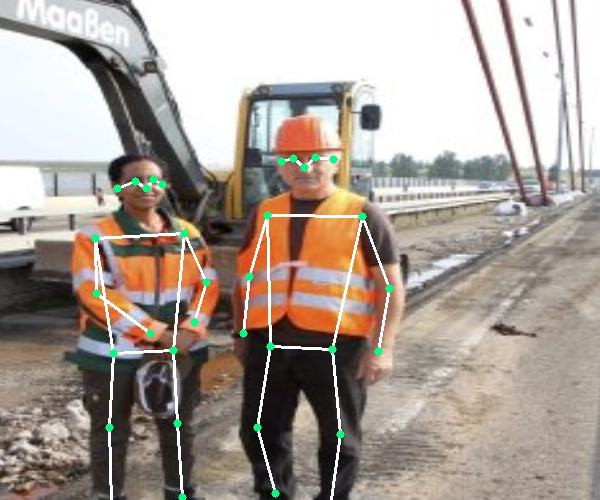
\includegraphics[width=\linewidth, valign=t]{figures/landmark1_crop_600x500.jpg} &
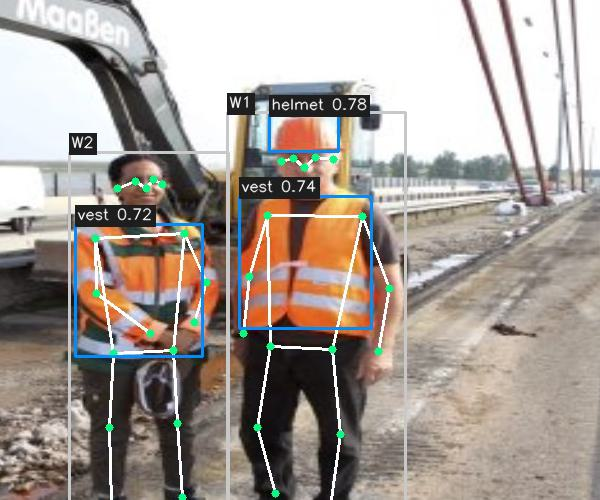
\includegraphics[width=\linewidth, valign=t]{figures/pact1_crop_600x500.jpg} &
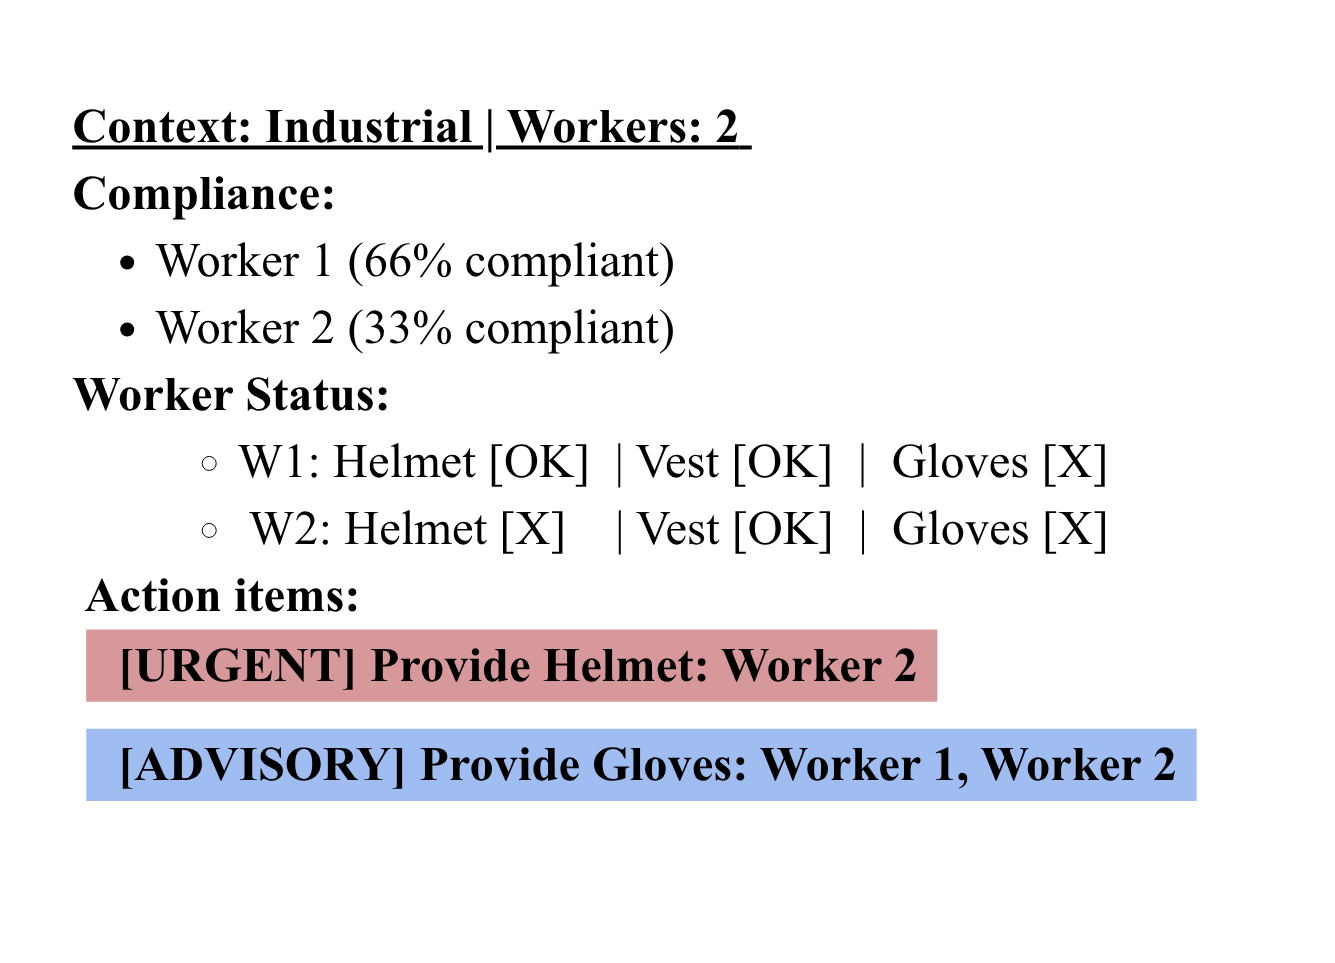
\includegraphics[width=\linewidth, valign=t]{figures/report1 (2).png} \\ \hline

% Baris CPPE-5
\rule{0pt}{10pt}
\textbf{CPPE-5} &
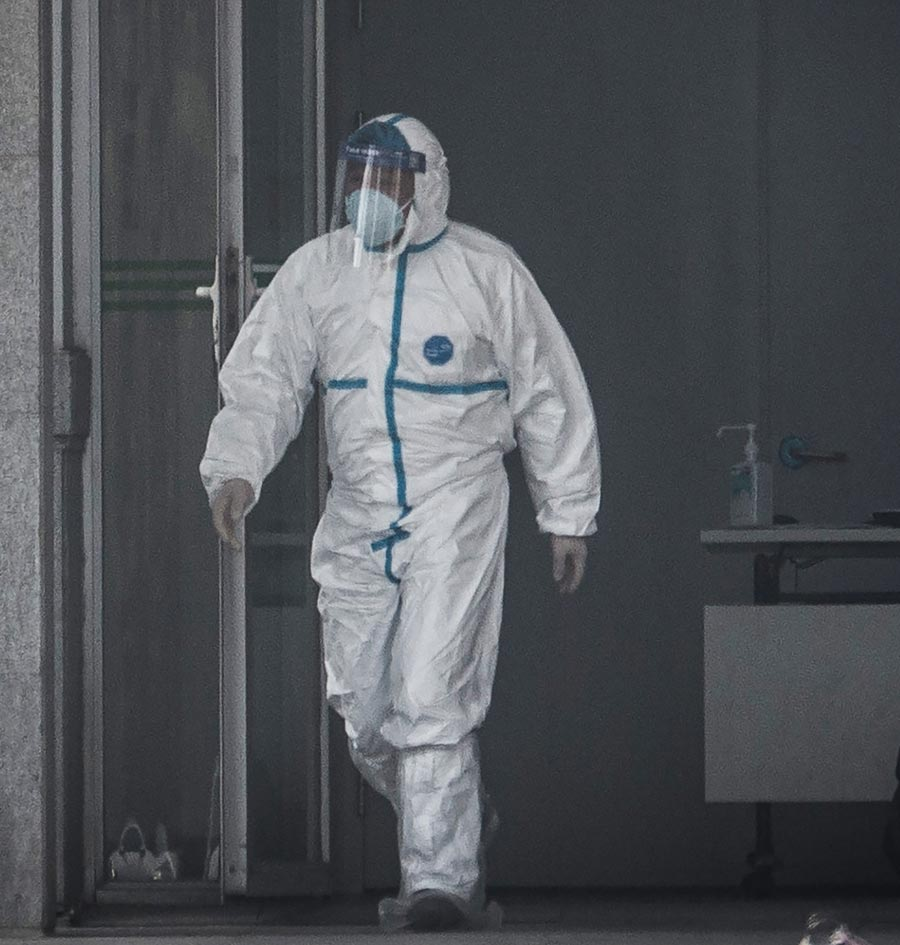
\includegraphics[width=\linewidth, valign=t]{figures/raw2.png} &
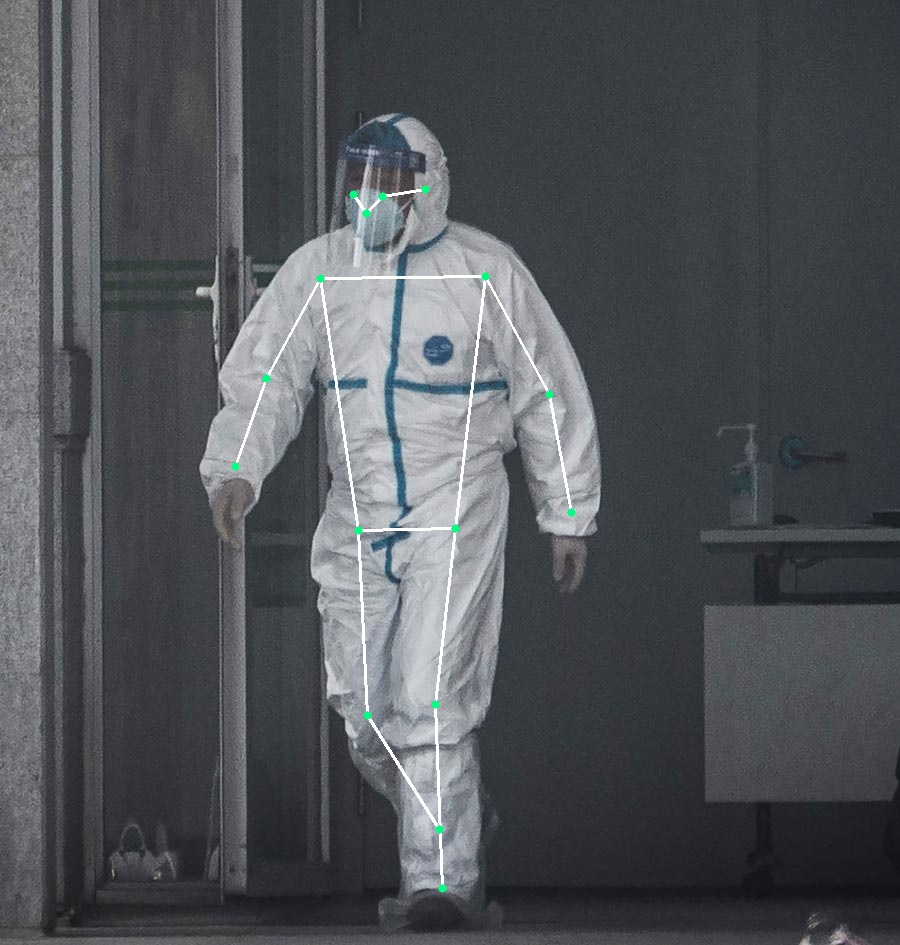
\includegraphics[width=\linewidth, valign=t]{figures/landmark2.jpg} &
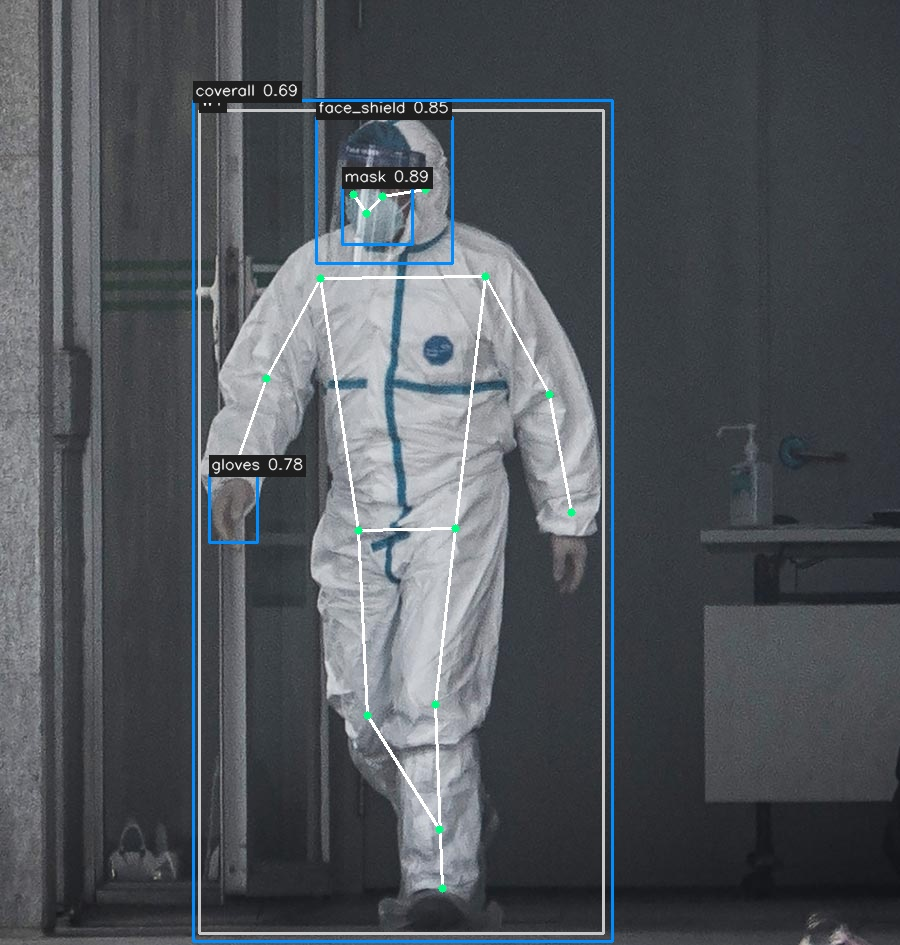
\includegraphics[width=\linewidth, valign=t]{figures/pact2.jpg} &
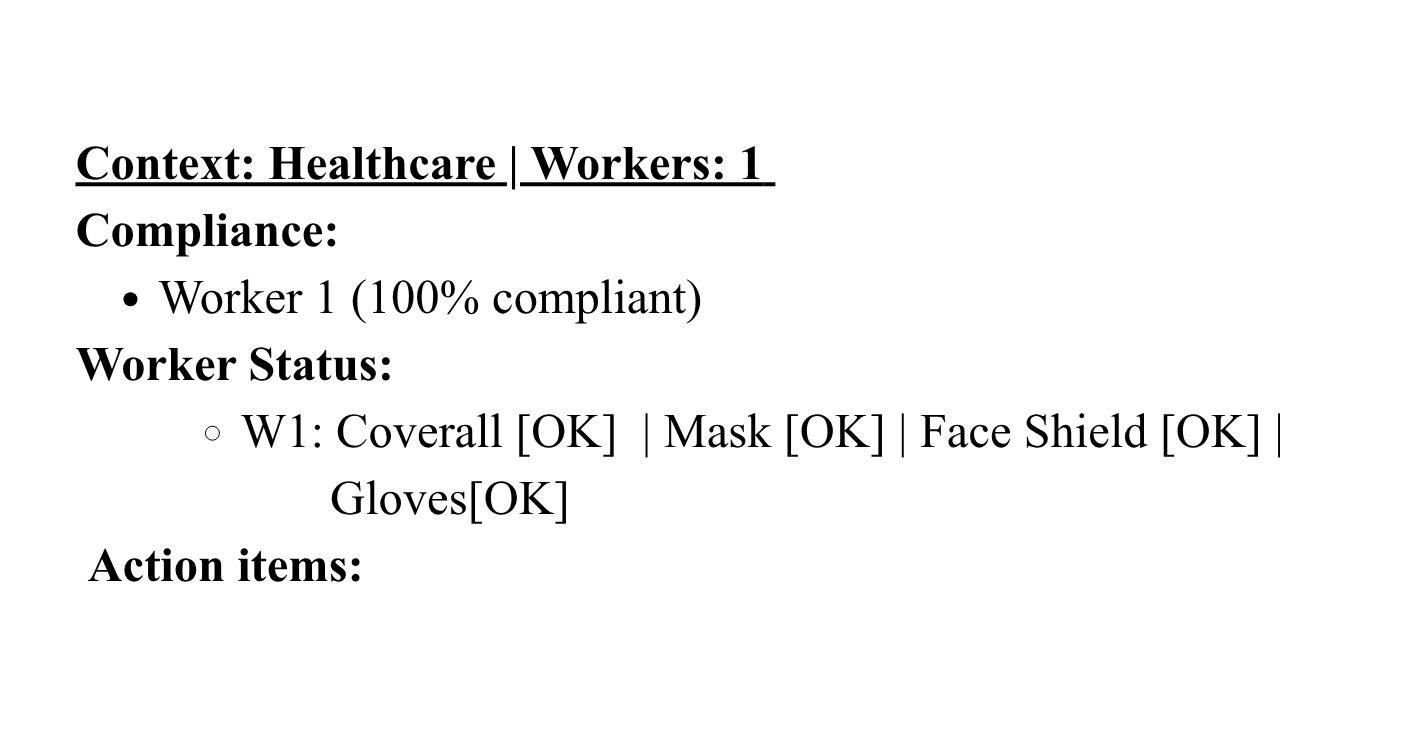
\includegraphics[width=1.1\linewidth, valign=t]{figures/report2 (2).png} \\ \hline

% Baris SH17
\rule{0pt}{10pt}
\textbf{SH17} &

\includegraphics[width=\linewidth, valign=t]{figures/raw3.jpeg} &
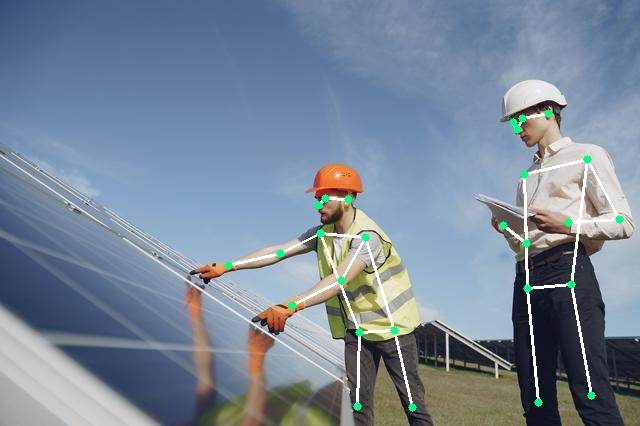
\includegraphics[width=\linewidth, valign=t]{figures/landmark3.jpg} &
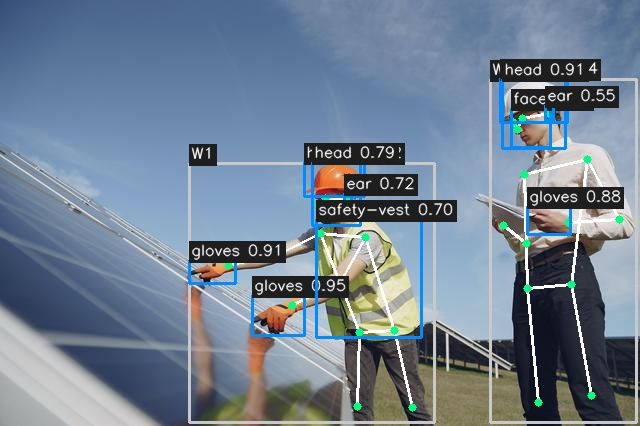
\includegraphics[width=\linewidth, valign=t]{figures/pact3.jpg} &
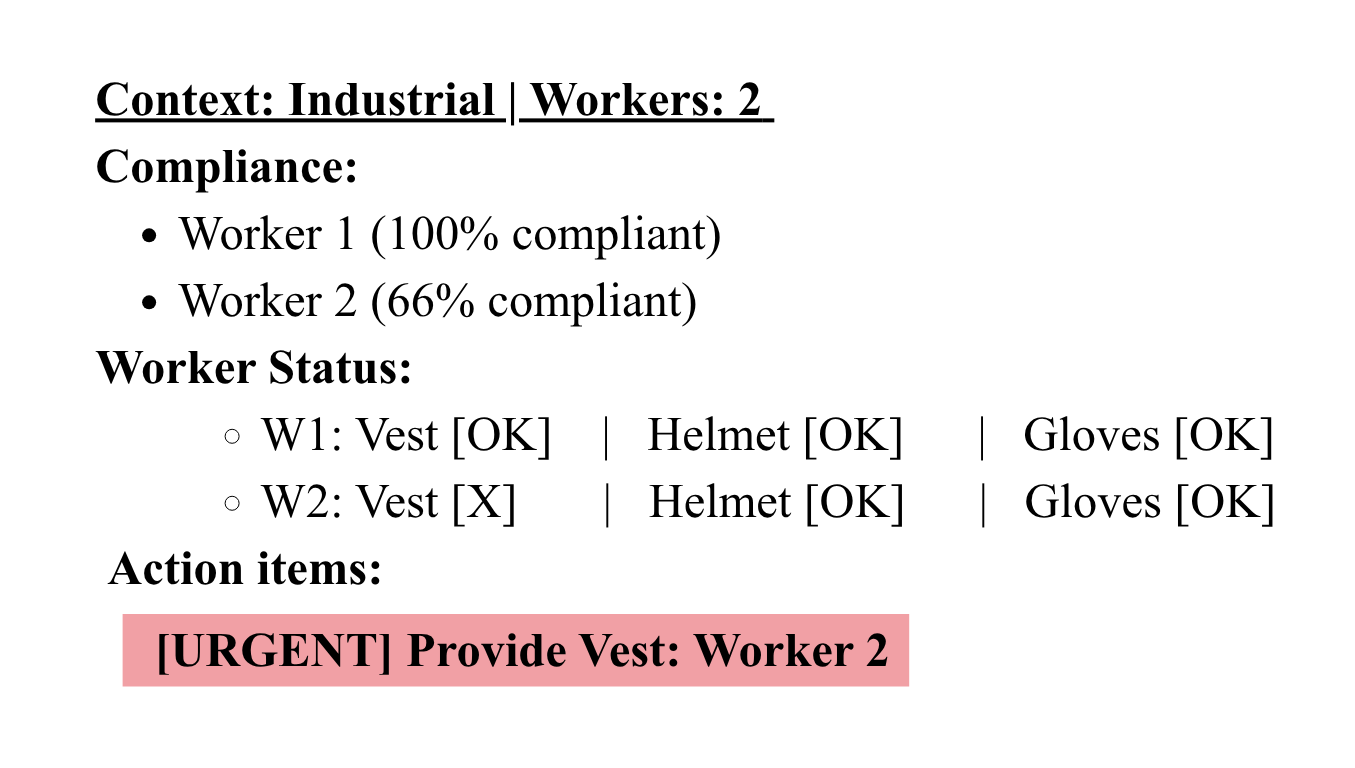
\includegraphics[width=\linewidth, valign=t]{figures/result3.png} \\ \hline

\end{tabular}
\end{table*}


\subsection{Compliance Reporting}
Earlier PPE compliance systems produce a single binary safety label for the entire scene~\cite{wen_automated_2024}, which is insufficient for multi-person environments where individual accountability is required. Systems that check compliance separately for each detected person represent a step toward per-worker granularity~\cite{fahmi2023enhanced}, and pipelines that identify missing PPE at the individual level provide the specific information needed for worker records~\cite{vukicevic2022compliance}. However, none of these works formalize a per-person compliance score or produce severity-tiered corrective action items linked to worker identifiers, leaving targeted safety audits and longitudinal compliance tracking unsupported.

Table~\ref{tab:related_comparison} summarizes the key characteristics of representative prior systems. The comparison covers pose integration strategy, per-person PPE attribution, compliance score granularity, severity-tiered reporting, and dataset domain. Two dimensions distinguish PACT from these prior systems: pose is used for assignment rather than filtering, and the system produces fractional per-person compliance scores with severity-tiered corrective action items rather than binary pass/fail outputs or scene-level labels.



\section{Method}


\subsection{Datasets}
Three publicly available datasets covering distinct deployment domains are used for evaluation. CHV \cite{ref5} contains 1,330 construction site images annotated across six classes (person, safety vest, and four helmet colors), evaluated under the original split (1,064/133/133 train/val/test). CPPE-5 \cite{ref1} contains 1,029 images across five medical PPE classes (coverall, face shield, gloves, goggles, mask), evaluated under the original split (1,000 train / 29 test); the dataset contains no person-class annotations. SH17 \cite{ref2} contains 8,099 industrial images annotated across 17 classes covering both body parts and PPE items, it is evaluated under the original split (6,479 train / 1,620 validation, used as test). All images are resized to $640 \times 640$ pixels prior to inference.


\subsection{System Overview}
PACT processes a single input image through three sequential stages, as illustrated in Fig.~\ref{fig:pipeline} and exemplified by Table~\ref{tab:qualitative_results}. In Stage~1 (Parallel Inference), a YOLO26L object detector and a YOLOv8x-pose model run simultaneously on the same input. YOLO26L produces a set of PPE bounding boxes, each labeled with a class and confidence score. YOLOv8x-pose independently localizes each person in the scene and extracts a skeleton of 17 body keypoints per person in COCO format.

In Stage~2 (Pose-Anchored Assignment), the PACT assignment module takes the PPE detections from YOLO26L and the skeletal keypoints from YOLOv8x-pose as input. For each detected PPE item, the module constructs anatomical body regions from the keypoints of each person and determines which person the item most plausibly belongs to using spatial overlap reasoning. This produces a set of per-person PPE attributions rather than a scene-level list of detected items.

In Stage~3 (Compliance Evaluation and Reporting), a rule-based module evaluates each worker's attributed PPE against a dataset-specific required set, computes a fractional compliance score per person, and generates a structured violation report with severity-tiered corrective action items.


\subsection{PPE Detection Module}
PPE detection uses YOLO26L \cite{sapkota_yolo26_2026}, a large-scale YOLO26 variant pretrained on COCO and fine-tuned per dataset. The model contains 24.75M parameters at 86.1~GFLOPs. Training uses AdamW ($\eta_0 = 1{\times}10^{-3}$, weight decay $5{\times}10^{-4}$), batch size~8, up to 150 epochs with early stopping at patience~20, and Automatic Mixed Precision (AMP). Augmentations include mosaic, horizontal flip, HSV jitter, random scale and translation, RandAugment, and random erasing. Each detection carries a bounding box, class label, and confidence score. Sub-threshold and person-class detections are discarded, as person localization is delegated to the pose module.


\subsection{Person and Pose Detection Module}
Person localization and keypoint extraction use YOLOv8x-pose \cite{yaseen_what_2024}, applied in inference mode without fine-tuning. It jointly detects persons and regresses 17 COCO-format skeletal keypoints per person, each with normalized coordinates and a visibility confidence score. Since undetected persons cannot receive PPE attribution, detection rate directly bounds assignment coverage. The extracted keypoints serve as geometric anchors for the assignment stage.


\subsection{PPE to Person Assignment}
The assignment module is the core contribution of PACT. It attributes each PPE detection to a specific worker using pose-anchored spatial reasoning, operating in two steps.


\subsubsection{Body Region Construction}
For each detected person, a set of anatomical body regions is constructed from their visible keypoints. Each PPE class maps to one or more regions based on its expected wearing location: helmets map to the head, vests to the torso, and gloves to the hands. Each region is defined as the bounding box enclosing its associated keypoints, expanded by a margin of $\delta$ times the region bounding box dimensions. A region is only constructed if at least two of its keypoints exceed a visibility threshold of 0.3, suppressing regions based on poorly localized estimates.


\subsubsection{IoU-Based Matching}
Each PPE detection is assigned to the person whose
anatomical body region produces the highest IoU with the
detection box. An assignment is accepted only if this IoU
exceeds $\tau_a = 0.10$. This threshold is intentionally
lower than the standard detection-matching threshold of 0.50
because the overlap is computed between a PPE box and a
compact anatomical anchor region rather than between two
boxes describing the same object. Small wearable items such
as helmets, gloves, and masks typically occupy only a
limited portion of the corresponding body region, and a
higher threshold would reject geometrically valid
assignments. The threshold therefore functions as a
permissive acceptance gate, while final attribution is
determined by the maximum-overlap person match. In
multi-person scenes, each PPE item is assigned to at most
one worker; if two detections of the same class are assigned
to the same person, only the higher-confidence detection
is retained.



\subsection{Compliance Scoring and Reporting}
After assigning detected PPE items to individual workers, the compliance evaluation module computes a per-person compliance score defined as the ratio of confirmed worn items to the total required equipment for that deployment context.  Required PPE sets are defined per dataset based on applicable regulations: helmet and vest for CHV (OSHA 29~CFR~1926.100, ISO~20471); coverall, mask, and gloves for CPPE-5 (WHO/CDC infection control guidelines); and helmet, safety-vest, and gloves for SH17 (OSHA 29 CFR 1926, ISO 45001).  A score of $1.0$ indicates full compliance, while partial compliance is tracked separately from a binary pass/fail classification.  The scene-level compliance rate is computed as the mean of all per-person scores.

For each worker, every missing required item is converted into a corrective action item.  Each action item is prefixed with \texttt{[URGENT]} or \texttt{[ADVISORY]} based on a static severity tier assigned to the PPE class.  Four tiers are defined: \textit{Critical} (helmet, hard hat), \textit{High} (vest, coverall, mask), \textit{Medium} (gloves, face shield, goggles), and \textit{Low} (shoes, protective suits).  A missing item at the Critical or High tier receives \texttt{[URGENT]}; Medium or Low receives \texttt{[ADVISORY]}.  Formally, for a missing class $c$,

\begin{equation}
u(c) =
\begin{cases}
\texttt{URGENT}   & \tau(c) \in \{\textsc{Critical}, \textsc{High}\} \\
\texttt{ADVISORY} & \text{otherwise}
\end{cases}
\end{equation}

where $\tau\colon \mathcal{C} \to \{\textsc{Critical}, \textsc{High}, \textsc{Medium}, \textsc{Low}\}$ is the severity mapping.  Action items are sorted by descending severity before output, so that the highest-risk violations appear first.

The reporting module merges these results into a structured output containing per-person compliance scores, the list of identified missing items, a scene-level summary, and the severity-sorted corrective action items grouped by worker identifier.


\subsection{Implementation Details}
YOLO26L is fine-tuned independently on each dataset split from COCO-pretrained weights. All experiments are conducted on an NVIDIA GeForce RTX~4050 Laptop GPU (6~GB VRAM) under CUDA~11.8, PyTorch~2.7, and Ultralytics~8.4.31.

For person localization and keypoint extraction, YOLOv8x-pose is applied in inference mode without fine-tuning on any target dataset. The model produces 17 skeletal keypoints per detected person in COCO body format, represented as $(x, y, v)$ where $v$ denotes visibility confidence. PACT assignment uses an anchor-overlap threshold $\tau_a = 0.10$, keypoint visibility threshold $\tau_v = 0.3$, and body region expansion margin $\delta = 0.10$ (10\% of the enclosing keypoint bounding box dimensions) across all datasets.


\subsection{Evaluation Metrics}
The evaluation framework is structured across three stages corresponding to the PACT pipeline. Stage~1 covers parallel inference, with person detection and PPE detection evaluated separately. For Stage~1a, YOLOv8x-pose is evaluated against ground-truth person bounding boxes at IoU threshold 0.50, reporting precision, recall, F1-score, and TP/FP/FN counts. For Stage~1b, YOLO26L is evaluated against ground-truth PPE bounding boxes at IoU threshold 0.50, reporting mAP50 and mAP50-95 for comparison with prior benchmarks \cite{ref5,ref1,ref2}.

Stage~2 evaluates PPE-to-person assignment accuracy on multi-person frames containing at least two ground-truth persons. CHV and SH17 do not provide explicit person-PPE relationship labels; therefore, ground-truth pairs are derived geometrically. Each ground-truth PPE box is paired with the ground-truth person box that covers the largest fraction of the PPE box, and PPE boxes with no meaningful person overlap are excluded. A matched detection (IoU $\geq 0.50$ with its ground-truth PPE item) is counted as correctly assigned if PACT attributed it to the same derived ground-truth person. CPPE-5 is excluded from this Stage~2 metric because it has no person-class ground-truth boxes. Let $A$ denote the number of correctly assigned detections and $T$ the total number of matched detections across all qualifying frames. Assignment accuracy is defined as:

\begin{equation}
    \text{Acc}_{\text{assign}} = \frac{A}{T}
    \label{eq:assign_acc}
\end{equation}

End-to-end latency is measured on the CPPE-5 test set by timing the PPE detection stage, the pose detection stage, and the anchor construction and compliance stage independently. Three warmup images are discarded before measurement. Latency is reported as the mean over all 29 test images.

Stage~3 does not introduce a dedicated metric; compliance scores and violation reports are evaluated qualitatively through the structured outputs.

\FloatBarrier


\section{Results and Discussion}
\FloatBarrier


\subsection{Performance on Stage~1}
Table~\ref{tab:l1a} shows person detection results for YOLOv8x-pose. CHV achieves F1 of 0.850 with precision 0.907 and recall 0.800. SH17 achieves the highest F1 of 0.887 with precision 0.944, though 448 persons remain undetected across 1,620 images, indicating that worker density increases missed detections despite high per-detection accuracy. CPPE-5 reaches F1 of only 0.483, with low precision (0.396). Displayed in Table~\ref{tab:l1b}, CHV mAP50 achieves 0.923 and mAP50-95 of 0.548, while CPPE-5 and SH17 achieve 0.765 and 0.652 respectively for mAP50.

\begin{table}[!htbp]
    \centering
    \caption{Person Detection Performance of YOLOv8x-Pose}
    \label{tab:l1a}
    \begin{tabular}{lcccrrr}
        \hline
        \textbf{Dataset}&
        \textbf{Precision} & \textbf{Recall} & \textbf{F1} &
        \textbf{TP} & \textbf{FP} & \textbf{FN} \\
        \hline
        CHV    & 0.907 & 0.800 & 0.850 & 360 & 37  & 90  \\
        SH17   & 0.944 & 0.836 & 0.887 & 2286 & 136 & 448 \\
        CPPE-5 & 0.396 & 0.618 & 0.483 & 21  & 32  & 13  \\
        \hline
        \multicolumn{7}{l}{\footnotesize TP: True Positive, FP: False Positive, FN: False Negative}
    \end{tabular}
\end{table}

\begin{table}[!htbp]
    \centering
    \caption{Overall PPE Detection Performance of YOLO26L}
    \label{tab:l1b}
    \begin{tabular}{lccccc}
        \hline
        \textbf{Dataset} &
        \textbf{Test Images} &
        \textbf{mAP50} & \textbf{mAP50-95} &
        \textbf{Precision} & \textbf{Recall} \\
        \hline
        CHV    & 133   & 0.923 & 0.548 & 0.926 & 0.859 \\
        CPPE-5 & 29    & 0.765 & 0.527 & 0.812 & 0.698 \\
        SH17   & 1,620 & 0.652 & 0.432 & 0.746 & 0.590 \\
        \hline
    \end{tabular}
\end{table}

Fig.~\ref{fig:map_loss} shows the mAP50 and Loss over epochs of YOLO26L across all dataset splits. mAP50 converges steadily and validation loss decreases across all splits, with no significant overfitting.

\begin{figure}[!htbp]
    \centering
    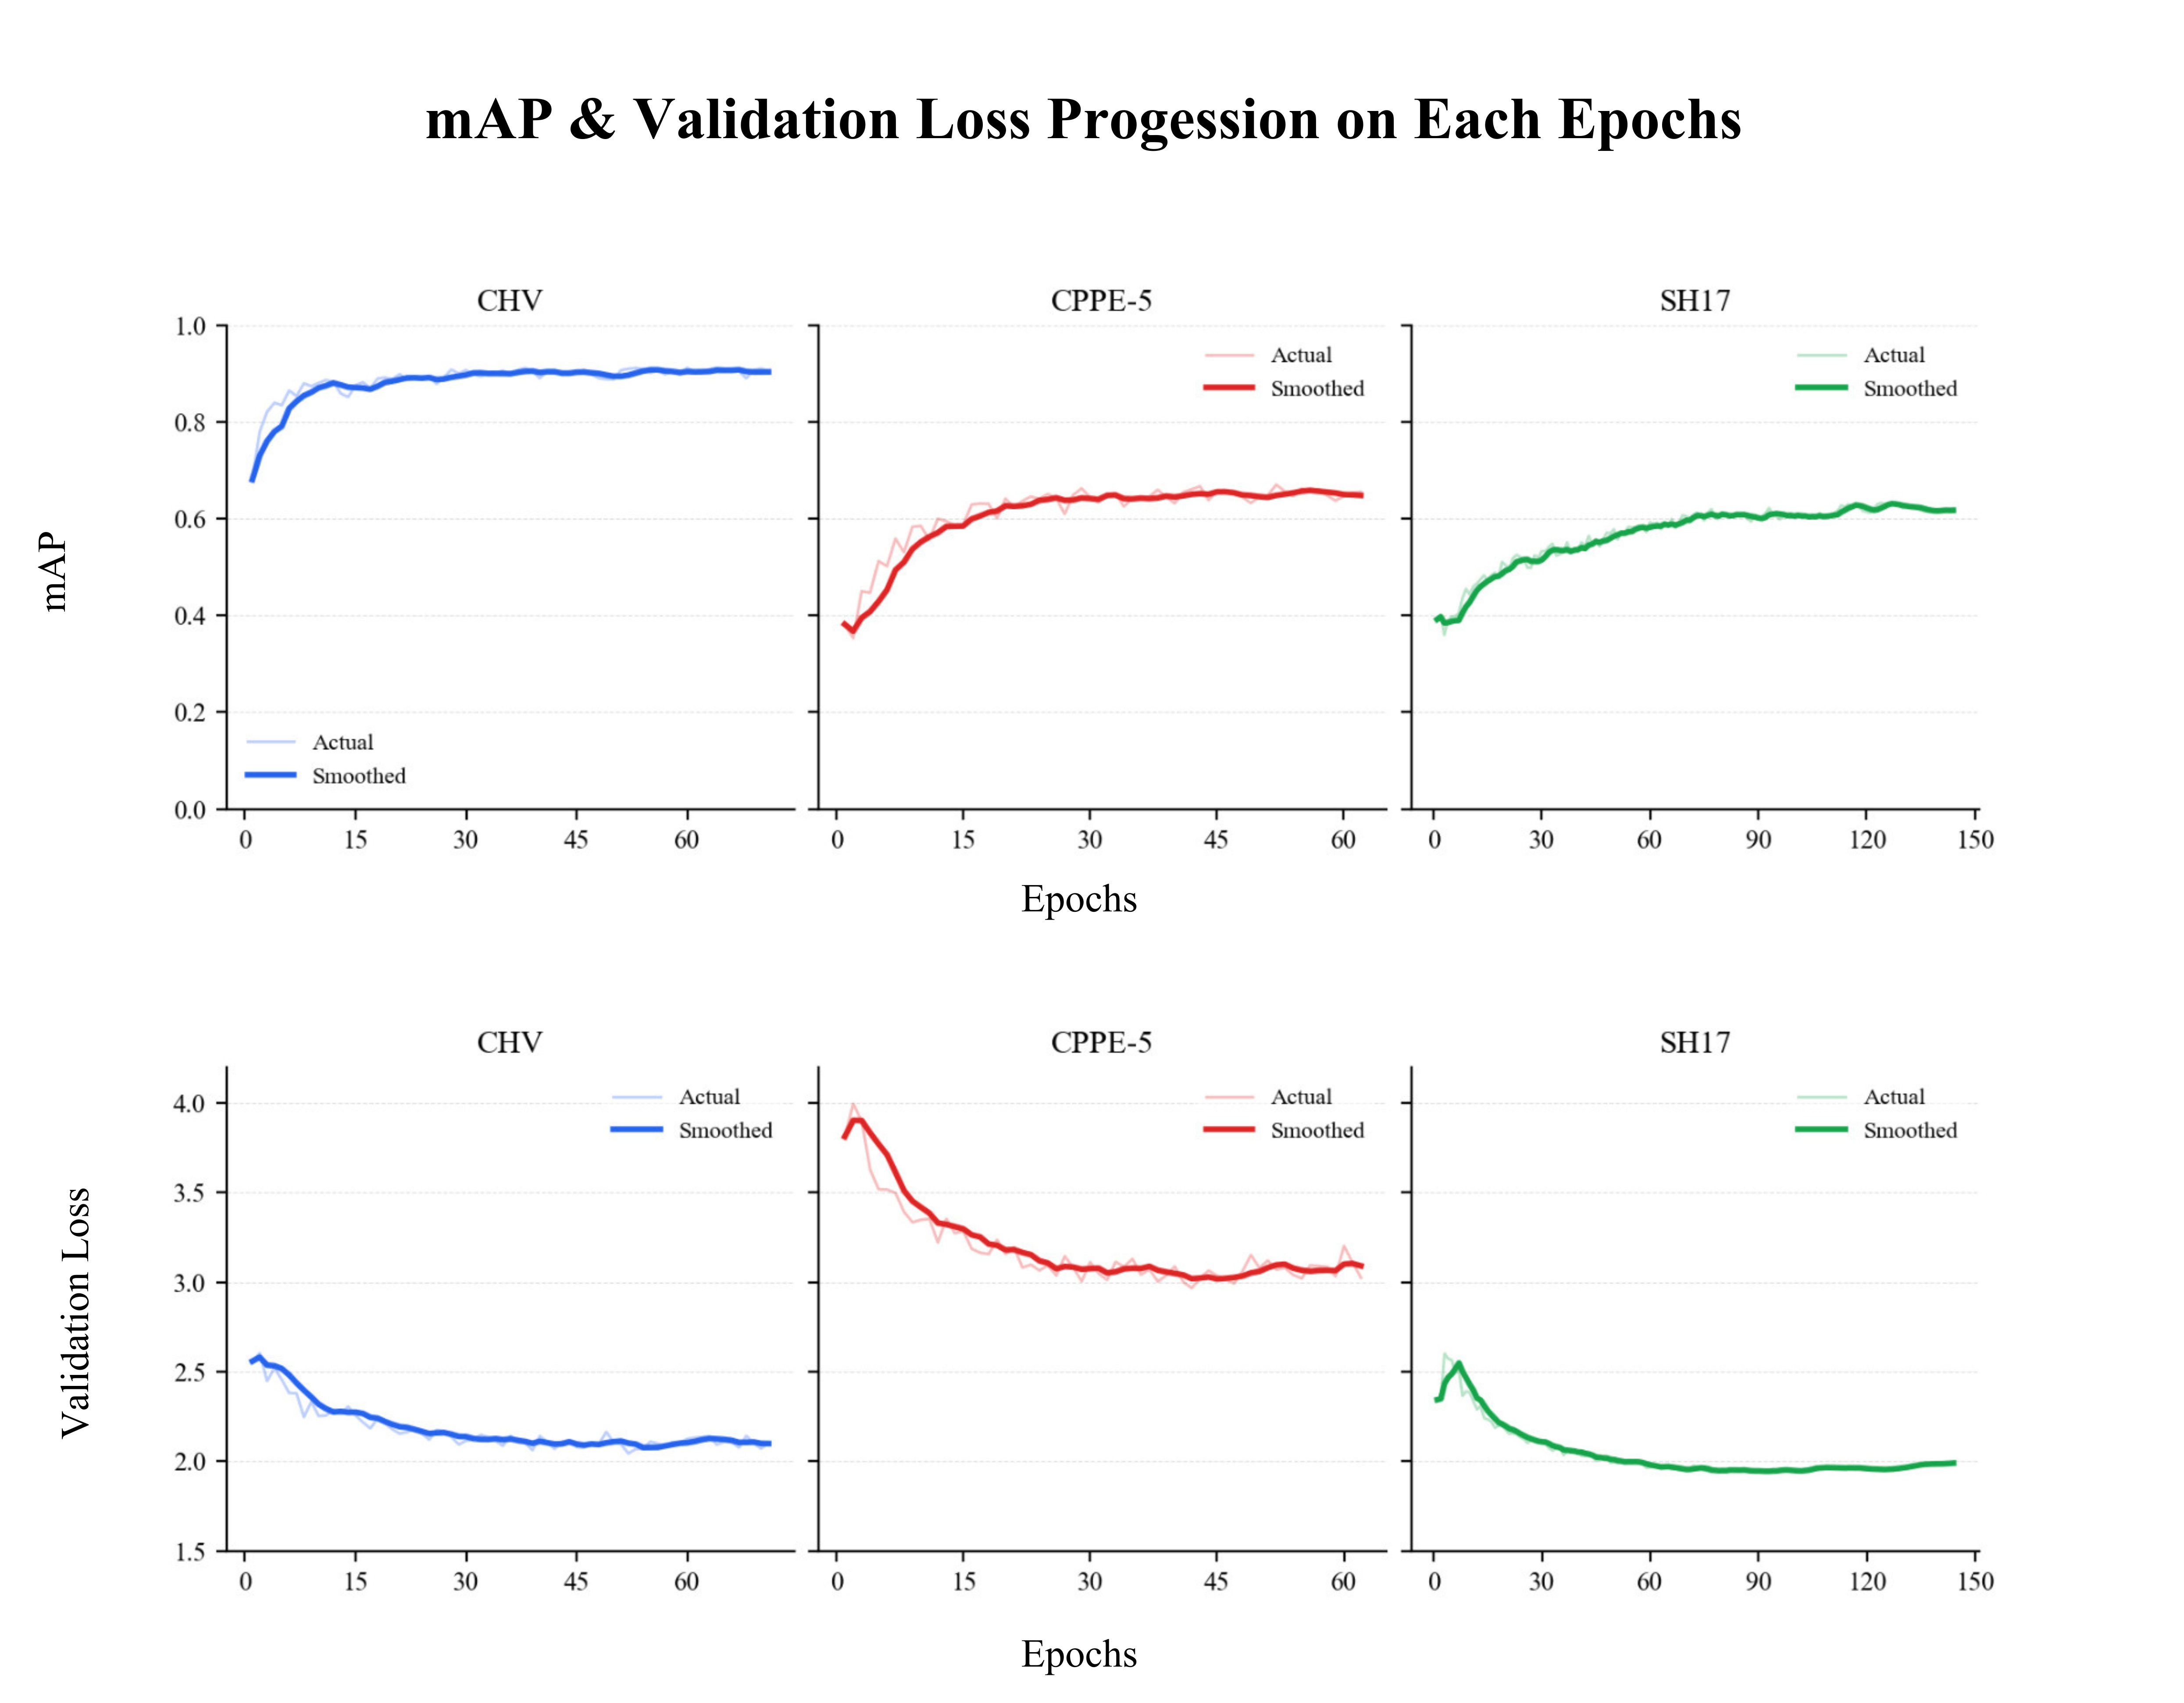
\includegraphics[width=\linewidth]{figures/maploss.png}
    \caption{Training performance of YOLO26L showing mAP50 and validation loss over epochs.}
    \label{fig:map_loss}
\end{figure}

Fig.~\ref{fig:error_cases} illustrates representative detection failures across datasets. On CHV and SH17, safety vests are missed because side-view perspectives reduce the visible area of the vest below the detector's confidence threshold. On CPPE-5, false detections occur in background regions for mask and coverall classes, indicating that the model activates on background patches with color similar to the typical mask and coverall in the dataset.

\begin{figure}[!htbp]
    \centering
    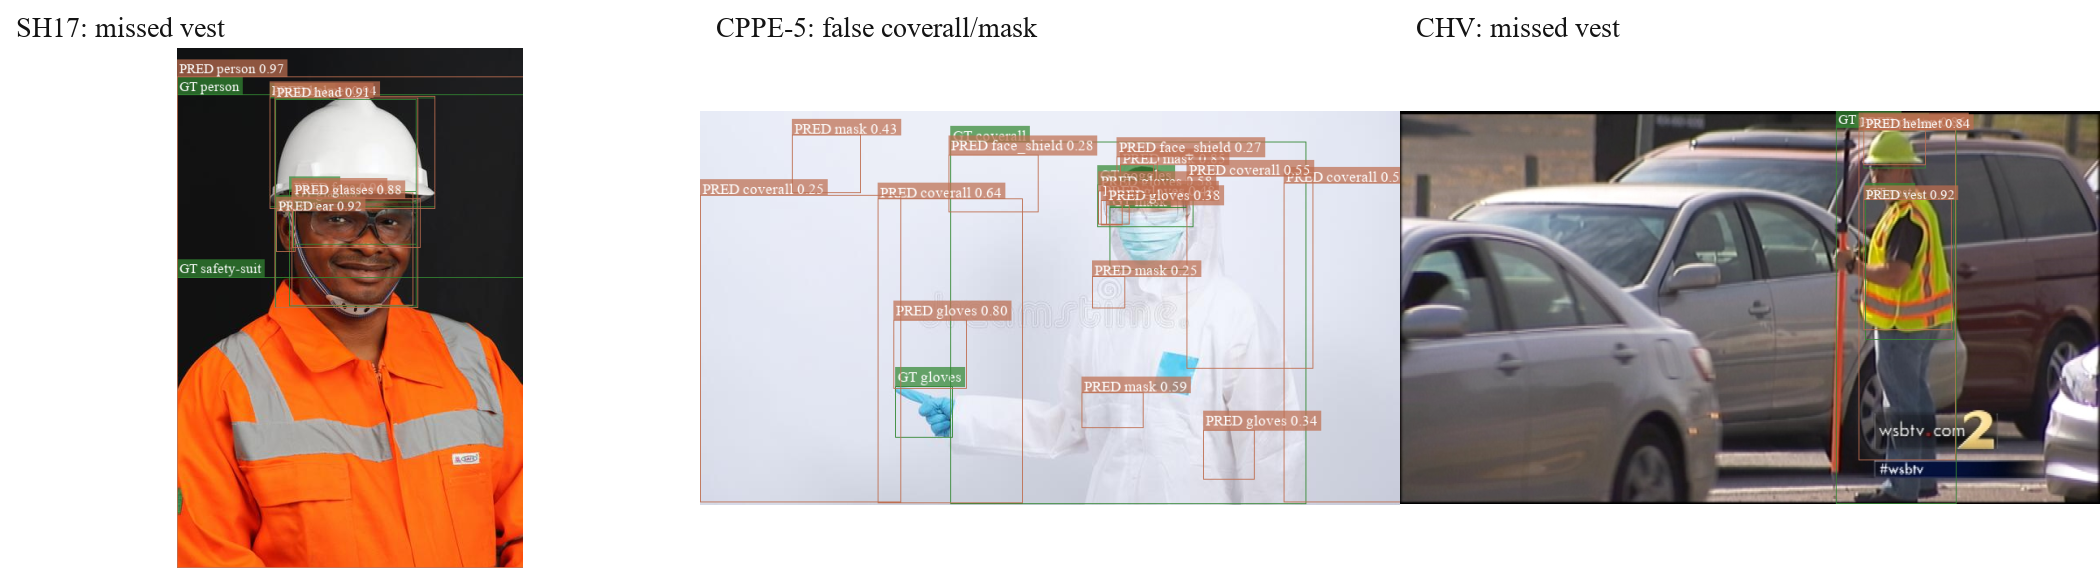
\includegraphics[width=\linewidth]{figures/wrongcase_annotated.png}
    \caption{Representative failure cases across datasets with explicit bounding-box callouts. Green bounding boxes are the ground truth, while the red bounding boxes are the predictions.
    CHV and SH17 show missed vest detections due to occlusion
    and side-view perspectives, while CPPE-5 exhibits false
    positives caused by background similarity.}
    \label{fig:error_cases}
\end{figure}


\subsection{Performance on Stage~2}
The accuracy of PPE-to-person assignment, shown in Table~\ref{tab:l2}, correlates with scene complexity. CHV achieves the highest accuracy (0.938) because construction scenes typically contain fewer overlapping workers and larger inter-person distances, which reduces ambiguity in body region IoU matching. SH17 yields a lower accuracy of 0.892, reflecting denser worker configurations where bounding boxes from adjacent persons often overlap and increase the probability of misassignment. CPPE-5 is not included in Table~\ref{tab:l2} because its annotations do not contain person boxes, making person-PPE assignment accuracy non-comparable without a derived proxy protocol.

\begin{table}[!htbp]
    \centering
    \caption{PPE-to-Person Assignment Accuracy}
    \label{tab:l2}
    \begin{tabular}{lccc}
        \hline
        \textbf{Dataset} &
        \textbf{Correct} & \textbf{Total} &
        \textbf{Accuracy} \\
        \hline
        CHV & 408 & 435 & 0.938 \\
        SH17& 521 & 584 & 0.892 \\
        \hline
        \multicolumn{4}{l}{\footnotesize CPPE-5 excluded because person ground-truth boxes are unavailable.} \\
    \end{tabular}
\end{table}


\subsection{Runtime Analysis}
Table~\ref{tab:runtime} reports mean latency per pipeline stage measured on the CPPE-5 test set ($n = 29$ images), with each stage timed independently in sequence. PPE detection accounts for 29.10~ms and pose detection for 45.84~ms; anchor construction and compliance evaluation account for 65.79~ms, making it the single largest contributor to total latency. Report generation (0.14~ms) is negligible. The mean end-to-end latency of 140.87~ms corresponds to 7.1~FPS, below the 25~FPS threshold commonly required for real-time video processing. The system is suited for batch or near-real-time inspection scenarios rather than continuous video monitoring.

\begin{table}[!htbp]
    \centering
    \caption{Mean Pipeline Latency on CPPE-5 Test Set}
    \label{tab:runtime}
    \begin{tabular}{lc}
        \hline
        \textbf{Stage} & \textbf{Mean Latency (ms)} \\
        \hline
        PPE detection (YOLO26L)          & 29.10 \\
        Pose detection (YOLOv8x-pose)    & 45.84 \\
        Anchor construction + compliance & 65.79 \\
        Report generation                &  0.14 \\
        \hline
        \textbf{Total}                   & \textbf{140.87} \\
        \hline
        \multicolumn{2}{l}{\footnotesize Mean FPS: 7.1 \quad
        GPU: NVIDIA RTX~4050 Laptop (6~GB)}
    \end{tabular}
\end{table}


\subsection{Limitations}
Several limitations exist in the proposed pipeline. Detection errors in Stage~1 propagate directly into the compliance report. Undetected PPE items are recorded as missing equipment, producing false non-compliance outputs that are indistinguishable from genuine violations at the reporting stage. Conversely, false positive detections may generate incorrect worn-item attributions, inflating compliance scores. The reporting module has no mechanism to distinguish between detection failure and actual non-compliance.

The assignment module is susceptible to misattribution in dense scenes where workers are in close proximity. When PPE bounding boxes spatially overlap multiple person regions, body region IoU matching may assign an item to the incorrect worker.

Finally, the system operates on individual frames without temporal context. It does not track workers across frames or maintain compliance state over time, limiting its applicability to continuous video-based reporting scenarios.



\section{Conclusion}
Detection-only PPE compliance systems cannot attribute equipment items to specific workers in multi-person scenes, limiting their utility in real deployments. PACT addresses this by combining YOLO26L-based PPE detection, YOLOv8x-pose-based person localization, and pose-anchored body region IoU assignment, with a rule-based module generating per-person compliance scores and severity-tiered reports. Evaluated across construction, medical, and industrial datasets under a three-stage protocol, PACT achieves mAP50 of 0.923 on CHV and 0.652 on SH17, and assignment accuracy of 0.938 on CHV and 0.892 on SH17 for datasets with person ground truth. End-to-end latency of 140.87~ms (7.1~FPS) positions PACT for batch and near-real-time inspection scenarios. Future work will address person detection coverage in crowded and occluded scenes such as CPPE-5, and extend the framework to video-based temporal tracking.


\bibliographystyle{IEEEtran}
\bibliography{reference}

\end{document}
